%%%%%%%%%%%%%%%%%%%%%%%%%%%%%%%%%%%%%%%%%%%%%%%%%%%%%%%%%%%%%%%%%%%%%%
% How to use writeLaTeX: 
%
% You edit the source code here on the left, and the preview on the
% right shows you the result within a few seconds.
%
% Bookmark this page and share the URL with your co-authors. They can
% edit at the same time!
%
% You can upload figures, bibliographies, custom classes and
% styles using the files menu.
%
%%%%%%%%%%%%%%%%%%%%%%%%%%%%%%%%%%%%%%%%%%%%%%%%%%%%%%%%%%%%%%%%%%%%%%


\documentclass[12pt]{article}
\usepackage[utf8]{inputenc}
\usepackage[T1]{fontenc}
\usepackage[brazil]{babel}
\usepackage{enumitem}
\usepackage{sbc-template}

\usepackage{graphicx,url}

\usepackage[brazil]{babel}   
\usepackage[utf8]{inputenc}  
\usepackage{enumitem}

     
\sloppy

\title{WireSense}

\author{Vitor Melchioretto\inst{1},Yuji Yamada Correa\inst{2}}


\address{Universidade do Estado de Santa Catarina
  (UDESC)\\
  Rua Paulo Malschitzki, 200 -- 89.219-710 -- Joinville -- SC -- Brazil
  \email{vitor.melchioretto@edu.udesc.br, xxx@xxx.xx.x}
}

\begin{document} 

\maketitle



%--------------------------------------------------------------------------------------------
\section{Introdução}
%
{Em processos industriais de fabricação de fios, eventos de rompimento interrompem o processo e geram retrabalho, descarte de material, tempo adicional de regulagem e mobilização de equipes de manutenção e qualidade. A dificuldade associada a esses eventos não reside apenas em detectá-los, mas em avaliar qual é a sua origem mais provável.}
%

%
{Essa identificação é dificultada pela multiplicidade de fatores que podem causar o evento, entre eles desvios no comportamento operacional das máquinas, variações de regulagem, degradação de componentes, variações de matéria-prima entre lotes e entre fornecedores, e efeitos combinados do contexto de operação. A avaliação da causa depende da experiência dos especialistas, o que reduz a padronização do diagnóstico e limita a sua escala para o volume de ocorrências da operação.}
%

%
{As informações disponíveis sobre o comportamento das máquinas e sobre os eventos que interrompem a produção permitem o uso de diferentes famílias de técnicas de ciência de dados. Uma família opera sobre o comportamento operacional das máquinas a partir de dados sensoriais. Outra responde por análises descritivas do histórico de eventos, organizadas em torno das entidades de produção associadas a cada ocorrência. A escolha de cada família depende da estrutura da fonte de dados e do tipo de pergunta que ela é capaz de sustentar.}
%

%
{Este artigo discute a estratégia de ciência de dados aplicável a esse problema, com foco nas escolhas de técnicas que se ajustam à natureza das tabelas disponíveis. A discussão organiza as técnicas em torno do tipo de dado sobre o qual cada uma opera, justifica a opção por abordagens não supervisionadas a partir da ausência de rótulo de causa no nível do evento, e descreve uma arquitetura que integra os resultados das técnicas em um diagnóstico da origem provável do rompimento. O escopo é metodológico, sem avaliação empírica em uma instalação específica.}
%--------------------------------------------------------------------------------------------

\section{Dados disponíveis}
%
{A discussão metodológica proposta na introdução começa pela apresentação dos dados que a operação efetivamente disponibiliza. A fábrica fornece, para esta pesquisa, duas tabelas que descrevem aspectos distintos do processo, com naturezas e granularidades próprias. A forma como cada uma chega define o tipo de transformação necessária antes que qualquer técnica de análise possa ser aplicada sobre ela. Esta seção descreve as duas tabelas no formato em que são recebidas e as operações de preparação que tornam o conjunto utilizável. As Figuras 1 e 2 apresentam uma representação visual de cada uma delas, na mesma ordem em que aparecem nas subseções a seguir.}
%

\begin{figure}[ht]
\begin{minipage}[b]{0.5\linewidth}
    \centering
    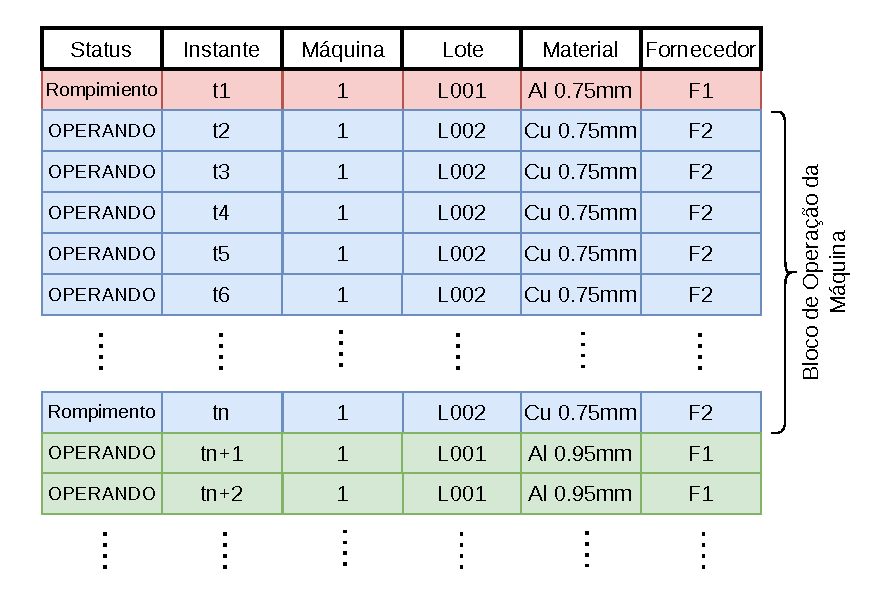
\includegraphics[width=1\linewidth]{Figuras/TabelaStatus.pdf}
    \caption{Representação visual da tabela de Status}
    \label{fig:tabelastatus}
\end{minipage}%
\begin{minipage}[b]{0.5\linewidth}
     \centering
    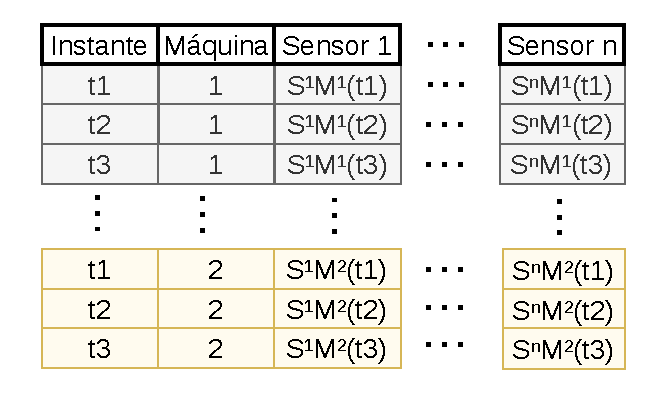
\includegraphics[width=1\linewidth]{Figuras/Sensores.pdf}
    \caption{Representação visual da tabela de Sensores}
    \label{fig:tabelasensores}
\end{minipage}
\end{figure}

%
\subsection{Tabela de status}
%
{A primeira tabela, ilustrada pela Figura~\ref{fig:tabelastatus}, registra o histórico de status de cada máquina ao longo do tempo. Cada linha corresponde a um intervalo de operação contínua ou a um evento discreto que interrompeu essa operação. As colunas nativas trazem o identificador do programa associado à execução, o nome do centro de máquina, o código e a descrição do evento, o tipo do evento, o instante inicial, o instante final e a duração do intervalo. A descrição do evento assume valores como \textsc{`OPERANDO'} para os intervalos de produção sem incidente e valores específicos para cada tipo de parada, incluindo categorias associadas a rompimentos por causas como bolha, asperidade e instabilidade de forno.}
%

%
{Atributos de produção como lote, material e fornecedor não fazem parte da tabela bruta. Eles foram incorporados por cruzamento temporal com a tabela de ordens de produção, e a Figura~\ref{fig:tabelastatus} já apresenta a tabela com essa união aplicada. Cabe ressaltar que a granularidade visual continua a mesma da tabela bruta. Cada linha representa um intervalo da máquina, e os eventos de rompimento aparecem como linhas pontuais dentro de um fluxo majoritariamente composto por intervalos de operação contínua.}
%

\subsection{Tabela de sensores}
%
{A segunda tabela representada pela Figura~\ref{fig:tabelasensores} é gerada pelo sistema de aquisição instalado nas máquinas e contém as leituras das variáveis monitoradas. Ela chega em formato longo, no qual cada linha registra uma leitura individual de um sensor, com identificação da variável de processo, do centro de máquina, do instante de registro e dos valores agregados máximo, médio e mínimo associados ao intervalo amostral. O conjunto de variáveis monitoradas cobre grandezas físicas e elétricas que descrevem o estado térmico, o estado mecânico e o estado elétrico da linha, incluindo temperaturas em diferentes pontos do recozedor, do forno e da zona de cura, tensões aplicadas em pontos críticos do percurso do fio, a velocidade da linha e medidas associadas aos ventiladores que controlam o ambiente térmico do forno.}
%

{Esse formato é adequado para o armazenamento, mas não para a análise multivariada das séries, que opera sobre matrizes nas quais cada linha representa um instante e cada coluna representa uma variável. Para tornar a tabela utilizável pelos métodos descritos na próxima seção, ela foi submetida a duas operações de preparação. A primeira foi um \textit{pivot} do formato longo para o formato largo, no qual cada coluna passa a corresponder a uma variável sensorial e cada linha a um instante. A segunda foi o preenchimento das lacunas temporais resultantes, executado com estratégia diferenciada conforme a cardinalidade de cada variável. A Figura~\ref{fig:tabelasensores} apresenta a tabela já no formato pivotado e com as lacunas tratadas, no estado em que ela alimenta as análises posteriores.}
%

\subsection{Transformações aplicadas antes da análise}
%
{A passagem das duas tabelas brutas para o formato consumido pelos métodos de análise envolve um conjunto de operações de preparação. A tabela de status passa por dois movimentos. Primeiro, recebe os atributos de produção provenientes da tabela de ordens, por meio de um cruzamento temporal que associa cada intervalo da máquina ao lote, ao material e ao fornecedor em produção naquele momento. Segundo, é filtrada para isolar os eventos discretos de rompimento, separando as linhas com descrição \textsc{`OPERANDO'} das linhas que representam paradas físicas. Da combinação dessas duas operações resulta uma tabela de eventos puros, que serve às análises de risco por lote, material e fornecedor.}
%

%
{A tabela de sensores passa por três movimentos. Primeiro, sofre o \textit{pivot} do formato longo para o formato largo, no qual cada linha passa a representar um instante e cada coluna passa a representar uma variável monitorada. Segundo, recebe um tratamento de lacunas temporais, executado por uma estratégia dupla. Variáveis com cardinalidade alta, que caracterizam grandezas contínuas, recebem interpolação linear entre as leituras válidas mais próximas. Variáveis com cardinalidade baixa, que caracterizam comportamento discreto, recebem propagação do último valor conhecido para frente, com propagação para trás aplicada como recurso residual. Terceiro, valores fisicamente inválidos de temperatura, abaixo do zero da escala adotada, são saneados antes da etapa de interpolação, para que não contaminem a estimativa das leituras vizinhas.}
%

%
{Ao final dessas transformações, as duas tabelas convergem para um formato compatível com os métodos descritos na próxima seção. A tabela de eventos passa a sustentar análises descritivas e estimativas de risco relativo agregadas por entidades de produção. A tabela de sensores passa a sustentar a caracterização do comportamento típico de cada combinação de máquina e material e a identificação de desvios em relação a esse comportamento. A ausência, em ambas as tabelas, de um rótulo confiável que indique a causa de cada rompimento é o elemento que afasta o problema das técnicas supervisionadas tradicionais e o aproxima das abordagens não supervisionadas que a próxima seção discute.}
%--------------------------------------------------------------------------------------------

\section{Técnicas e justificativa}
%
{Esta seção organiza as famílias de técnicas de ciência de dados aplicadas ao problema, em torno do tipo de dado sobre o qual cada uma opera. Para cada família, descreve o que ela faz, por que ela cabe na tabela correspondente e o que ela não resolve.}
%

\subsection{Detecção de anomalias multivariada sobre as séries sensoriais}
%
{A tabela de sensores, após o tratamento descrito na seção anterior, representa o estado operacional de cada máquina ao longo do tempo. A análise busca identificar se o comportamento da máquina no entorno de um rompimento destoa do padrão observado quando ela operava sem incidente sobre o mesmo material. Trata-se de detecção de anomalias em séries multivariadas sem rótulo, sustentada por abordagem não supervisionada.}
%

%
{O algoritmo escolhido é o \textit{Isolation Forest}~\cite{Liu2008}, baseado em ensembles de árvores de isolamento. Ele aprende partições aleatórias do espaço das variáveis monitoradas e atribui a cada observação um escore proporcional à facilidade de isolá-la das demais. Observações fáceis de isolar tendem a ser raras na distribuição treinada e recebem escores compatíveis com anomalia. A escolha se apoia em três propriedades. O algoritmo opera de forma não supervisionada, o que se ajusta à ausência de rótulo identificada na seção anterior. Sua complexidade é linear no número de observações e independente da dimensionalidade efetiva das variáveis, o que torna o treinamento tratável em volumes industriais. E não assume distribuição paramétrica nas variáveis monitoradas, o que importa em um conjunto de medidas físicas com escalas e perfis distintos.}
%

{O treinamento é estratificado por combinação de máquina e material. Em vez de um modelo global, treina-se um \textit{Isolation Forest} independente para cada combinação observada, porque o comportamento operacional da máquina varia conforme o material processado. Misturar essas populações em um modelo único dilui o sinal de anomalia, já que o algoritmo passa a considerar normal a união dos padrões. A estratificação preserva o comportamento esperado de cada combinação, ao custo de exigir um histórico mínimo para cada uma.}
%

{O escore do \textit{Isolation Forest} é calculado por leitura, mas a unidade de análise é o bloco contínuo de operação, definido como um intervalo ininterrupto de produção da mesma máquina sobre o mesmo material, ordem e lote, sem retomada após parada. Cada bloco recebe um escore agregado, dado por uma estatística de cauda dos escores das leituras que o compõem, e em seguida transformado em percentil empírico contra o histórico de blocos da mesma combinação. A agregação reduz a sensibilidade a leituras isoladas e torna o escore comparável entre combinações de tamanhos distintos.}
%

{A associação entre cada rompimento e um bloco acontece \textit{a posteriori}. Para cada evento, busca-se o bloco de operação imediatamente anterior na mesma combinação de máquina e material, dentro de uma janela de tolerância. O bloco identificado fornece o contexto operacional do diagnóstico. Rompimentos sem bloco compatível ou sem modelo treinado recebem rótulos próprios, distintos do rótulo de ausência de anomalia.}
%

{Essa abordagem não resolve três questões. Não identifica qual sensor contribui para um escore alto, porque o escore agregado é multivariado e não decomposto por variável. Não estabelece relação causal direta entre o desvio operacional e o rompimento, apenas indica que o estado da máquina no entorno do evento era atípico para aquela combinação. E não cobre combinações de máquina e material sem histórico suficiente para o treinamento, o que limita a cobertura do método.}
%
\subsection{Estatística histórica de risco relativo sobre a tabela de eventos}
%
{A tabela de eventos, depois das transformações descritas na Seção 2, registra os rompimentos ocorridos na operação, com cada evento associado a um lote, um material e um fornecedor. A pergunta a responder é se algum desses agrupamentos apresenta frequência de rompimento acima da referência observada para o seu contexto.}
%

{A abordagem adotada é estatística descritiva sobre o histórico observado, sem qualquer modelo preditivo. A justificativa é direta. Como a tabela não traz rótulo confiável de causa por evento, não há alvo supervisionado para treinar um classificador. O que existe é o registro fatual de que rompimentos aconteceram em certos contextos, e a hipótese implícita de que contextos com taxa anormalmente alta de rompimento merecem investigação como suspeita de matéria-prima defeituosa. A análise traduz essa hipótese em uma medida quantitativa, sem afirmar causalidade, e devolve para o especialista uma classificação ordinal que ele pode interpretar e contestar.}
%

{O cálculo se organiza em torno de uma normalização por exposição. A taxa bruta de rompimento de um lote sobre um material é definida como o número de rompimentos atribuídos a esse lote dividido pelo número de horas em que o lote esteve em produção naquele material. Essa taxa bruta é então comparada com uma referência histórica do próprio material, calculada como a razão entre o total de rompimentos do material e o total de horas de exposição do material, agregada sobre todos os lotes observados. A razão entre a taxa do lote e a referência do material produz uma taxa relativa, adimensional, que expressa o quanto o lote rompe a mais ou a menos do que o esperado para aquele material. Lotes que processam mais de um material recebem uma taxa relativa final calculada como média ponderada das taxas relativas por material, com pesos proporcionais às horas de exposição em cada um.}
%

{A taxa relativa final é então traduzida em uma classificação por faixas, derivada do percentil empírico do lote na distribuição de todos os lotes analisados. Lotes acima de certo percentil entram em \textsc{ALTO RISCO}. Faixas intermediárias produzem \textsc{RISCO ELEVADO}, \textsc{RISCO NORMAL} e \textsc{BAIXO RISCO}. O uso de faixas em vez de um número contínuo serve a uma necessidade prática do laudo de produção, que precisa entregar ao especialista uma indicação acionável, e não um escore que ele teria que interpretar sozinho. Os cortes de percentil são parâmetros do sistema, centralizados e ajustáveis pelo time da fábrica conforme a calibração se refine no uso.}
%

{Há três coisas que essa abordagem não consegue afirmar. Não estabelece causalidade, apenas associação estatística. Um lote pode aparecer com taxa relativa alta por motivos que não têm a ver com a sua qualidade intrínseca, como atribuição equivocada de rompimento ou regulagens limítrofes da máquina. Não captura nenhum sinal sobre o estado operacional das máquinas, que é o domínio da análise descrita na Seção 3.1. E não cobre lotes com exposição muito baixa, que entram em uma faixa específica de \textsc{INDETERMINADO} porque a estimativa de taxa, com poucas horas, fica dominada pelo ruído amostral.}
%
\subsection{Pilar MP:}

\subsubsection{Unidade de Análise e Fontes de Dados}


\bibliographystyle{sbc}
\bibliography{sbc-template}

\end{document}
